%% SW design: PSoC Controllers
\begin{figure}[htbp] \centering
{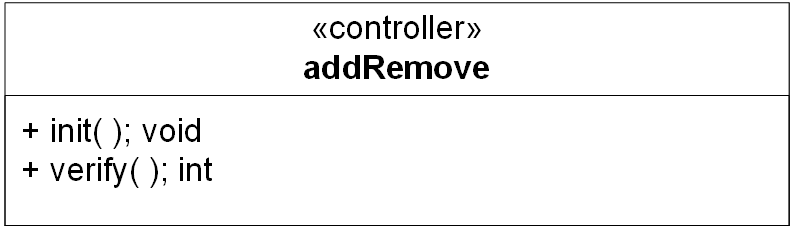
\includegraphics[scale=1.3]{filer/design/Klassediagrammer/sw_psoc_addRemove}}
\caption{Klasse addRemove}
\label{fig:sw_psoc_class_addremove}
\end{figure} 

{\centering
\textbf{addRemove}\par
}
\textbf{Ansvar:} Kontrollerer hændelsesforløbet ifm. usecase 1. \

\verb+void init( )+\\
\textbf{Parametre:} Ingen. \\
\textbf{Returværdi:} Ingen. \\
\textbf{Beskrivelse:} Har ingen funktionalitet.\\

\verb+int verify( )+\\
\textbf{Parametre:} Ingen. \\
\textbf{Returværdi:} 0 ved succes ellers negativ i overenstemmelse med fejl-listen. \\
\textbf{Beskrivelse:} Returnerer kun 0. Bruges til at verificerer kommunikation mellem Master og Enhed.\\

\begin{figure}[htbp] \centering
{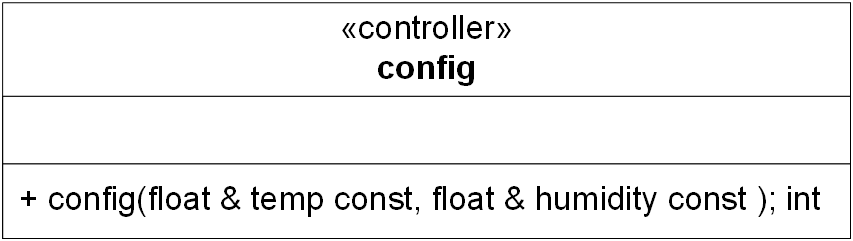
\includegraphics[scale=1.3]{filer/design/Klassediagrammer/sw_psoc_config}}
\caption{Klasse config}
\label{fig:sw_psoc_class_config}
\end{figure} 

{\centering
\textbf{config}\par
}
\textbf{Ansvar:} Kontrollerer hændelsesforløbet ifm. usecase 2. \

\textbf{Attributter:}
\begin{itemize}
	\item \verb+parameters * parametersPtr_+ Pointer til associeret objekt
	\item \verb+buffer * bufferPtr_+ Pointer til associeret objekt
\end{itemize}

\verb+void init( parameters *, buffer *)+\\
\textbf{Parametre:} Pointere til associerede objekter. \\
\textbf{Returværdi:} Ingen. \\
\textbf{Beskrivelse:} Sætter sine private pointere. \\

\verb+int config( const float * temp, const float * humi  )+ \\
\textbf{Parametre:} To pointere til hhv. temperatur og fugtighedsgrænser \\
\textbf{Returværdi:} 0 ved succes ellers negativ i overenstemmelse med fejl-listen. \\
\textbf{Beskrivelse:} Gemmer parametre i \verb+parameters+ objektet med metoderne \verb+setTemp()+ og \verb+setHumi()+. \\

\begin{figure}[htbp] \centering
{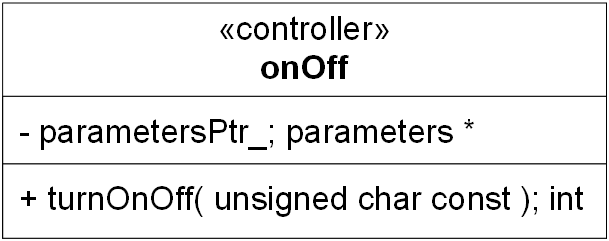
\includegraphics[scale=1.3]{filer/design/Klassediagrammer/sw_psoc_onOff}}
\caption{Klasse onOff}
\label{fig:sw_psoc_class_onOff}
\end{figure} 

{\centering
\textbf{onOff}\par
}
\textbf{Ansvar:} Kontrollerer hændelsesforløbet ifm. usecase 3. \

\textbf{Attributter:}
\begin{itemize}
	\item \verb+parameters * parametersPtr_+ Pointer til associeret objekt
	\item \verb+buffer * bufferPtr_+ Pointer til associeret objekt
\end{itemize}

\verb+void init( parameters *, buffer *)+\\
\textbf{Parametre:} Pointere til associerede objekter. \\
\textbf{Returværdi:} Ingen. \\
\textbf{Beskrivelse:} Sætter sine private pointere. \\

\verb+int turnOnOff( const unsigned char )+ \\
\textbf{Parametre:} 0 = off, 1 = on \\
\textbf{Returværdi:} 0 ved succes ellers negativ i overenstemmelse med fejl-listen. \\
\textbf{Beskrivelse:} Hvis modtaget parameter er inden for range sættes flaget \verb+active_+ i \verb+parameters+-objektet ud fra den modtagende parameter, ellers gemmes en fejl i \verb+buffer+-objektet. \\

\begin{figure}[htbp] \centering
{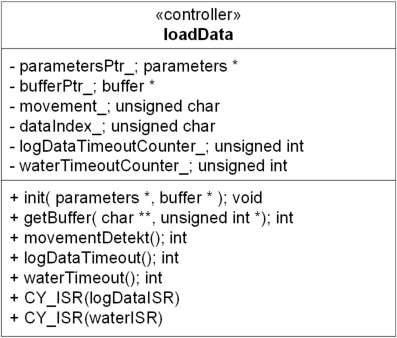
\includegraphics[scale=1.3]{filer/design/Klassediagrammer/sw_psoc_loadData}}
\caption{Klasse loadData}
\label{fig:sw_psoc_class_loadData}
\end{figure} 

{\centering
\textbf{loadData}\par
}
\textbf{Ansvar:} Kontrollerer hændelsesforløbet ifm. usecase 4. \

\textbf{Attributter:}
\begin{itemize}
	\item \verb+parameters * parametersPtr_+ Pointer til associeret objekt
	\item \verb+buffer * bufferPtr_+ Pointer til associeret objekt
	\item \verb+unsigned char movement_+ Flag for at huske på registreret bevægelse
	\item \verb+unsigned char dataIndex_+ Index til hvor data er gemt i bufferen 
	\item \verb+unsigned int logDataTimeoutCounter_+ Tæller til at forøge delaytiden ifm. datalogning
	\item \verb+unsigned int waterTimeoutCounter+ Tæller til at forøge delaytiden ifm. vandingsafbrydelse
\end{itemize}

\verb+void init( parameters *, buffer *)+\\
\textbf{Parametre:} Pointere til associerede objekter. \\
\textbf{Returværdi:} Ingen. \\
\textbf{Beskrivelse:} Sætter sine private pointere samt initialisere de andre medlemsdatatil 0. Sætter datalogningstimer i gang og sætter timerens ISR-callback til \verb+logDataISR+. Sætter også vandingsafbrydelsens ISR-callback til \verb+waterISR+. Laver en måling af data fra sensorene ved at kalde \verb+logDataTimeout()+. \\

\verb+int getBuffer( char ** buf, unsigned int len * )+ \\
\textbf{Parametre:} Pointer til at skrive adressen til bufferen i og en længde. \\
\textbf{Returværdi:} 0 ved succes ellers negativ i overenstemmelse med fejl-listen. \\
\textbf{Beskrivelse:} Kalder \verb+getData()+ i \verb+buffer+-objektet med de modtagende parametre.\\

\verb+int movementDetekt( )+ \\
\textbf{Parametre:} Ingen. \\
\textbf{Returværdi:} 0 ved succes ellers negativ i overenstemmelse med fejl-listen. \\
\textbf{Beskrivelse:} Henter \verb+active_+-flaget fra \verb+parameters+. Hvis den er aktiv, deaktiveres Enheden ved at sætte flaget til 0 og \verb+waterTimer+ startes. Flaget \verb+movement_+ sættes til 1. \\

\verb+int logDataTimeout( )+ \\
\textbf{Parametre:} Ingen. \\
\textbf{Returværdi:} 0 ved succes ellers negativ i overenstemmelse med fejl-listen. \\
\textbf{Beskrivelse:} Aflæser data fra sensorene i \verb+sensorPackage+. Henter grænseværdierne i \verb+parameters+. Gemmer de hentede data i \verb+buffer+-objektet. Afhængig af \verb+movement_+-flaget, tilføjes passende \verb+char+ efter målt data i hht. dataprotokollen, \ref{header:dataprotokol}, og flaget sættes til 0. Hvis den målte data er uden for grænserne aktiveres vanding ved at kalde \verb+water(1)+.\\

\verb+int waterTimeout( )+ \\
\textbf{Parametre:} Ingen. \\
\textbf{Returværdi:} 0 ved succes ellers negativ i overenstemmelse med fejl-listen. \\
\textbf{Beskrivelse:} Aktiverer vanding ved at sætte \verb+active_+-flaget til 1 i \verb+parameters+. Stopper \verb+waterTimer+. \\

\verb+CY_ISR(logDataISR)+ \\
\textbf{Parametre:} Ingen. \\
\textbf{Returværdi:} 0 ved succes ellers negativ i overenstemmelse med fejl-listen. \\
\textbf{Beskrivelse:} Hvis \verb+logDataTimeoutCounter_+ er større end grænsen \verb+LOGDATATIMEOUT+*1000/10.923, hvor konstanterne er defineret af \verb+logDataTimer+s clock-hastighed, nulstilles denne og \verb+logDataTimeout()+ kaldes.\\

\verb+CY_ISR(waterISR)+ \\
\textbf{Parametre:} Ingen. \\
\textbf{Returværdi:} 0 ved succes ellers negativ i overenstemmelse med fejl-listen. \\
\textbf{Beskrivelse:}  Hvis \verb+waterTimeoutCounter_+ er større end grænsen \verb+WATERTIMEOUT+*1000/10.923, hvor konstanterne er defineret af \verb+waterTimer+s clock-hastighed, nulstilles denne og \verb+waterTimeout()+ kaldes.\\
